\documentclass[11pt]{article}
\usepackage[margin=1in]{geometry}
\usepackage{lmodern}
\usepackage[T1]{fontenc}
\usepackage{microtype}
\usepackage{amsmath,amssymb,mathtools}
\usepackage{booktabs}
\usepackage{enumitem}
\usepackage{graphicx}
\usepackage{xcolor}
\usepackage[most]{tcolorbox}
\usepackage[colorlinks=true,linkcolor=blue!50!black,urlcolor=blue!50!black]{hyperref}

\definecolor{keyblue}{RGB}{30,70,140}
\newtcolorbox{keyidea}[1][]{colback=keyblue!5,colframe=keyblue!70,
  fonttitle=\bfseries,title=#1,boxrule=0.6pt,arc=2pt,left=6pt,right=6pt}
\newtcolorbox{caution}[1][]{colback=orange!6,colframe=orange!70!black,
  fonttitle=\bfseries,title=#1,boxrule=0.6pt,arc=2pt,left=6pt,right=6pt}

\newcommand{\E}{\mathbb{E}}
\newcommand{\mb}{\bar m}
\setlist{itemsep=2pt,topsep=4pt}
\graphicspath{{figures/}}

\title{\textbf{The Two Utilities of Problem 21}\\[4pt]
\large AMS 516 Project --- reference notes on CARA, Merton and the shortfall penalty}
\author{Deepak Singh}
\date{October 2026}

\begin{document}
\maketitle

\begin{abstract}
These notes compare the utility in the original statement of Problem 21 with the
shortfall-penalty utility of our proposal. They cover CARA utility and the Merton
position, explain why the original peer term has no effect on decisions when noise is
independent, and show how the shortfall penalty makes risk aversion depend on where an
investor stands relative to the population average. Numbers use the defaults in
\texttt{configs/base.yaml}: $r=0.02$, $\mu=0.08$, $\sigma=0.20$, $\gamma=1$, $\lambda=2$,
$T=1$, and the $\lambda=0$ equilibrium mean $\mb_T\approx1.1$.
\end{abstract}

\setcounter{tocdepth}{1}
\tableofcontents

%======================================================================
\section{The setup}

Each investor holds wealth $X_t$ and chooses a \emph{dollar amount} $\pi_t$ in the
stock; the rest earns the risk-free rate $r$:
\[
  dX_t = \bigl[rX_t + \pi_t(\mu-r)\bigr]\,dt + \pi_t\sigma\,dW_t .
\]
Each investor has their own Brownian motion $W_t$ (independent noise). At the horizon they
receive $U(X_T,\mb_T)$, where $\mb_T$ is the average terminal wealth of the population,
and they maximise $\E[U(X_T,\mb_T)]$. With a continuum of investors and independent noise,
$\mb_T$ is a deterministic number by the law of large numbers.

The two utilities are
\begin{align*}
  \text{original:}\quad & U(x,\mb) = -e^{-\gamma(x-\theta\mb)}
     = -e^{-\gamma x}\cdot e^{\gamma\theta\mb}, \\
  \text{proposed:}\quad & U(x,\mb) = -e^{-\gamma x}
     - \tfrac{\lambda}{2}\bigl((\mb-x)^+\bigr)^2 .
\end{align*}
Both are built on the same term $-e^{-\gamma x}$, which is CARA utility. They differ only
in how $\mb$ is attached to it.

%======================================================================
\section{CARA utility}

\textbf{CARA} stands for \emph{constant absolute risk aversion}: $U(x)=-e^{-\gamma x}$ with
$\gamma>0$. Absolute risk aversion is
\[
  A(x) = -\frac{U''(x)}{U'(x)} .
\]
For CARA, $U'=\gamma e^{-\gamma x}>0$ (more wealth is better) and
$U''=-\gamma^2e^{-\gamma x}<0$ (concave, so risk-averse), hence $A(x)=\gamma$ at every
wealth level.

What this implies:
\begin{itemize}
  \item \textbf{Wealth doesn't change attitudes to a fixed-dollar bet.} A $\pm\$1{,}000$
        gamble looks the same at \$10k as at \$10M.
  \item \textbf{The optimal stock holding is a fixed dollar amount} (Section~\ref{sec:merton}).
  \item \textbf{Negative wealth is allowed}, which fits our domain $x\in[-1,3]$.
  \item \textbf{Shifting wealth by a constant only rescales $U$:}
        $-e^{-\gamma(x-c)} = e^{\gamma c}\cdot(-e^{-\gamma x})$. This is the reason the
        original peer term has no effect (Section~\ref{sec:original}).
\end{itemize}

\begin{center}
\begin{tabular}{@{}lll@{}}
\toprule
 & CARA & CRRA (Problem 12) \\
\midrule
Formula & $-e^{-\gamma x}$ & $x^{1-\gamma}/(1-\gamma)$ \\
Constant quantity & absolute risk aversion $A=\gamma$ & relative risk aversion $xA(x)=\gamma$ \\
Optimal holding & fixed dollar amount & fixed fraction of wealth \\
Allowed wealth & all real $x$ & $x>0$ \\
\bottomrule
\end{tabular}
\end{center}
CRRA is more realistic (richer people take bigger dollar bets); CARA is far easier to
solve, which is why mean-field portfolio games usually use it.

%======================================================================
\section{The Merton position}\label{sec:merton}

The \textbf{Merton position} is the optimal dollar holding of a plain CARA investor, from
Merton's continuous-time portfolio problem (1969--71):
\[
  \boxed{\;\pi^*(t) = \frac{\mu-r}{\gamma\sigma^2}\,e^{-r(T-t)}\;}
\]
With our parameters $(\mu-r)/(\gamma\sigma^2) = 0.06/0.04 = 1.5$, so $\pi^*(T)=1.5$ and
$\pi^*(0)=1.5\,e^{-0.02}\approx1.47$.

\textbf{Where it comes from.} Over a short interval $dt$, holding $\pi$ in the stock adds
expected excess gain $\pi(\mu-r)\,dt$ and variance $\pi^2\sigma^2\,dt$. A CARA investor
trades them off as gain $-\tfrac{\gamma}{2}\times$variance, maximised at
$\pi=(\mu-r)/(\gamma\sigma^2)$. The factor $e^{-r(T-t)}$ appears because a dollar of risk
taken at time $t$ grows by $e^{r(T-t)}$ before $T$, so earlier on you hold slightly less to
carry the same terminal risk.

\textbf{Reading the pieces.} Higher reward $\mu-r$ means more stock; higher risk $\sigma^2$
or risk aversion $\gamma$ means less.

\textbf{Value function.} The expected utility from following the Merton position is
\[
  V(t,x) = -\exp\!\Bigl(-\gamma x\,e^{r(T-t)} - \tfrac12\kappa^2(T-t)\Bigr),
  \qquad \kappa = \frac{\mu-r}{\sigma}\ \text{(Sharpe ratio, $0.3$)} .
\]
In the code, \texttt{merton\_pi} is the position and \texttt{merton\_value} is this $V$
(\texttt{src/mfg/benchmarks.py}); \texttt{Params.kappa} is the Sharpe ratio.

%======================================================================
\section{The original utility: why the peer term does nothing}\label{sec:original}

The original utility factorises:
\[
  U(x,\mb) = \underbrace{e^{\gamma\theta\mb}}_{\text{positive constant}}
             \cdot\underbrace{\bigl(-e^{-\gamma x}\bigr)}_{\text{plain CARA}} .
\]
Under independent noise $\mb$ is a fixed number, so the first factor is a positive
constant. Multiplying a utility by a positive constant never changes which outcome is
preferred, so the optimal strategy is exactly the Merton position, for any $\theta$. The
same cancellation shows up in the risk aversion: $A(x)=\gamma$, with no $\theta$ and no
$\mb$ in it.

\begin{keyidea}[Consequence]
With independent noise the original game is trivial: $\mb$ doesn't affect anyone's choice,
so there is no feedback between individuals and the crowd. The peer term only becomes
active with \emph{common} noise, where $\mb_T$ is random and correlated with each
investor's own wealth.
\end{keyidea}

%======================================================================
\section{The proposed utility: a one-sided shortfall penalty}

\[
  U(x,\mb) = -e^{-\gamma x} - \tfrac{\lambda}{2}\bigl((\mb-x)^+\bigr)^2 .
\]
The penalty is \textbf{added}, not multiplied, and it depends on $x$, so it changes how
outcomes are ranked. It is \textbf{one-sided}: zero when $x\ge\mb$, and quadratic in the
shortfall $g=\mb-x$ below it. Beating the average earns no bonus; falling behind hurts.
This is like a fund manager's career risk.

Write $g=\mb-x$ for the shortfall. Above and below the average:
\begin{center}
\renewcommand{\arraystretch}{1.3}
\begin{tabular}{@{}lll@{}}
\toprule
 & $x\ge\mb$ & $x<\mb$ \\
\midrule
$U$   & $-e^{-\gamma x}$ & $-e^{-\gamma x}-\tfrac{\lambda}{2}g^2$ \\
$U'$  & $\gamma e^{-\gamma x}$ & $\gamma e^{-\gamma x}+\lambda g$ \\
$U''$ & $-\gamma^2e^{-\gamma x}$ & $-\gamma^2e^{-\gamma x}-\lambda$ \\
\bottomrule
\end{tabular}
\end{center}
Below the average each extra dollar is worth more, by $\lambda$ times the shortfall.

\begin{caution}[A kink at the average]
$U$ and $U'$ are continuous at $x=\mb$, but $U''$ jumps by $\lambda$. Finite-difference
grids and PINN collocation points need to resolve this, and the terminal-condition loss is
hardest to fit there.
\end{caution}

\begin{figure}[p]
  \centering
  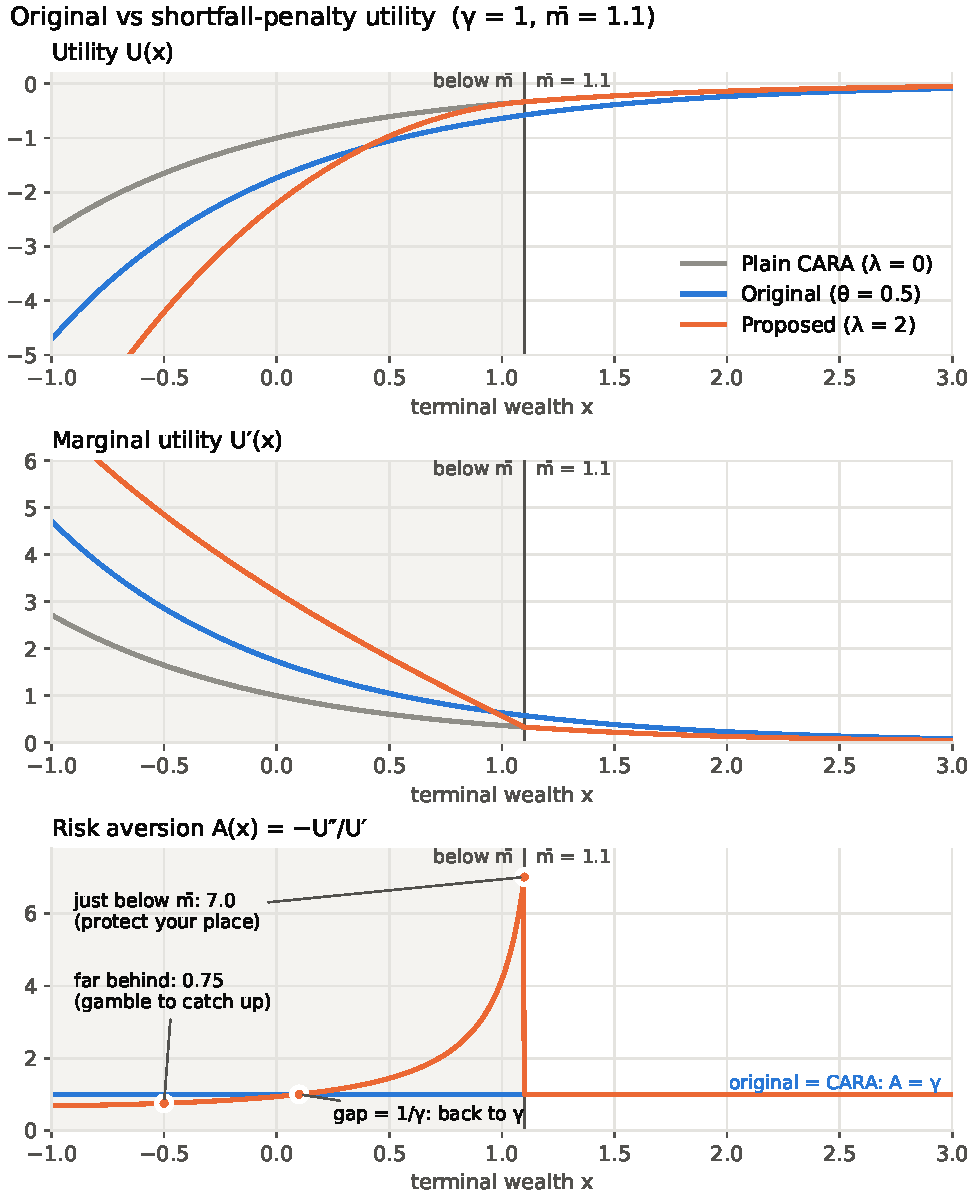
\includegraphics[width=\textwidth]{utility_comparison.pdf}
  \caption{Plain CARA (gray), the original utility with $\theta=0.5$ (blue) and the proposed
  utility with $\lambda=2$ (orange), for $\gamma=1$, $\mb=1.1$. The shaded region is
  wealth below $\mb$. Blue is gray rescaled; in the risk-aversion panel the two coincide.
  Made with \texttt{scripts/plot\_utilities.py -{}-stacked}.}
  \label{fig:utilities}
\end{figure}

%======================================================================
\section{Risk aversion, and where the 7 comes from}

Above the average, $A(x)=\gamma$ as for CARA. Below it,
\[
  A(x) = \frac{\gamma^2e^{-\gamma x}+\lambda}{\gamma e^{-\gamma x}+\lambda g},
  \qquad g = \mb - x > 0 .
\]

\textbf{Just below the average ($g\to0$).} The penalty's slope $\lambda g$ vanishes, but its
curvature $\lambda$ does not:
\[
  A(\mb^-) = \frac{\gamma^2e^{-\gamma\mb}+\lambda}{\gamma e^{-\gamma\mb}}
           = \gamma + \frac{\lambda e^{\gamma\mb}}{\gamma}
           = 1 + 2e^{1.1} = 1 + 2(3.004) \approx 7.0 .
\]
The numerator of $A$ jumps when crossing $\mb$ while the denominator doesn't, which gives
the vertical spike in Figure~\ref{fig:utilities}.

Equivalently, compare the two curvatures at $\mb$: the penalty's is $\lambda=2$ and CARA's
is $\gamma^2e^{-\gamma\mb}=e^{-1.1}\approx0.333$. Their ratio is the
\emph{penalty strength}
\[
  s = \frac{\lambda}{\gamma^2e^{-\gamma\mb}} \approx 6.0,
  \qquad A(\mb^-) = \gamma(1+s) = 7 .
\]
So just below the average the investor is 7 times as risk-averse as plain CARA. The 7 is
not special: it grows with $\lambda$, and with $\mb$, because CARA's own curvature is
smaller at higher wealth.

\textbf{Crossover at $g=1/\gamma$.} Setting $A=\gamma$ gives
$\gamma^2e^{-\gamma x}+\lambda=\gamma^2e^{-\gamma x}+\lambda\gamma g$, i.e.\ $g=1/\gamma$,
whatever the value of $\lambda$. Beyond that gap $A<\gamma$: the investor is
\emph{less} risk-averse than CARA.

%======================================================================
\section{From risk aversion to positions}

At $t=T$ the optimal position is
\[
  \pi^*(T,x) = \frac{\mu-r}{\sigma^2}\cdot\frac{U'(x)}{-U''(x)}
             = \underbrace{\frac{\mu-r}{\gamma\sigma^2}}_{\text{Merton}=1.5}\cdot\frac{\gamma}{A(x)} .
\]
Wherever $A(x)$ differs from $\gamma$, the position differs from Merton by the factor
$\gamma/A(x)$:

\begin{center}
\begin{tabular}{@{}lrrrl@{}}
\toprule
Position & $x$ & gap $g$ & $A(x)$ & $\pi^*(T,x)$ \\
\midrule
Above the average   & $1.1^+$ & 0    & 1.00 & 1.50 \quad (Merton) \\
Just below          & $1.1^-$ & 0    & 7.01 & 0.21 \quad (protect your place) \\
Slightly behind     & 0.6     & 0.5  & 1.65 & 0.91 \\
Crossover           & 0.1     & 1.0  & 1.00 & 1.50 \\
Far behind          & $-0.5$  & 1.6  & 0.75 & 1.99 \quad (gamble to catch up) \\
Very far behind     & $-1.0$  & 2.1  & 0.68 & 2.20 \\
\bottomrule
\end{tabular}
\end{center}

\begin{keyidea}[Three regimes]
Above the average, behave like CARA. Slightly behind, become very cautious and hug the
average. Far behind (gap beyond $1/\gamma$), take \emph{more} risk than Merton. The
original utility can't produce any of this: its $A(x)$ is flat.
\end{keyidea}

%======================================================================
\section{The HJB: same equation, different terminal condition}

By the dynamic programming principle and It\^o's formula, the value function
$V(t,x)=\sup_\pi\E[U(X_T,\mb_T)\mid X_t=x]$ satisfies
\[
  V_t + \sup_\pi\Bigl\{\bigl[rx+\pi(\mu-r)\bigr]V_x + \tfrac12\pi^2\sigma^2V_{xx}\Bigr\} = 0,
  \qquad V(T,x) = U(x,\mb_T).
\]
The first-order condition gives $\pi^* = -(\mu-r)V_x/(\sigma^2V_{xx})$, and substituting back,
\[
  V_t + rxV_x - \frac{(\mu-r)^2}{2\sigma^2}\,\frac{V_x^2}{V_{xx}} = 0 .
\]
This PDE is the \textbf{same for both utilities}; only the terminal condition differs. For
the original utility (and for $\lambda=0$) it has the closed form of
Section~\ref{sec:merton}, multiplied by $e^{\gamma\theta\mb}$ in the original case. At
$t=T$ the first-order condition reduces to the position formula of the previous section.

%======================================================================
\section{Why $\lambda=0$ is the benchmark}

Setting $\lambda=0$ gives plain CARA, which under independent noise behaves exactly like the
original utility for any $\theta$. Everything is then explicit:
\begin{itemize}
  \item position $\pi^*(t)=1.5\,e^{-r(T-t)}$ and the value function of
        Section~\ref{sec:merton};
  \item population mean $\E[X_t]=e^{rt}+0.09\,t\,e^{r(t-T)}$, so $\mb_T\approx1.110$;
  \item population variance $0.04\,e^{2rt}+0.09\,t\,e^{2r(t-T)}$.
\end{itemize}
Every solver (finite differences, Monte Carlo, PINNs) must reproduce these before its
$\lambda>0$ results can be trusted; \texttt{tests/test\_benchmarks.py} checks them.

For $\lambda>0$, $\mb$ sets where the kink sits. Each investor's choice depends on $\mb$,
and $\mb$ is the average of everyone's resulting wealth. That loop is a genuine fixed point,
which is what the coupled HJB--Fokker--Planck system solves.


\end{document}
